Auch wenn keine Verbesserung zu erwarten ist, soll dieser Teilerfolg nun ein Bild übertragen werden.
Dabei wird immerhin ersichtlich, wie das Vorgehen auf zwei Dimensionen erweitert werden kann.

Ein schwarz-weiss Bild kann man als Matrix betrachten, dessen Einträge zwischen 0 und 1 für die Helligkeit eines Pixels stehen.
0 entspricht schwarz, 1 entspricht weiss.

Als Versuchsbild wird ein etwas verschwommenes Dreieck, wie abgebildet links in \ref{deconvolve:example} (ohne blauen und orange Linie) verwendet.
Die Grösse beträgt $9600\times9600$ Pixel, analog den 9600 Samples der Funktion $f(x)$ aus Abbildung \ref{deconvolve:1d}.
\begin{figure}[h]
\centering
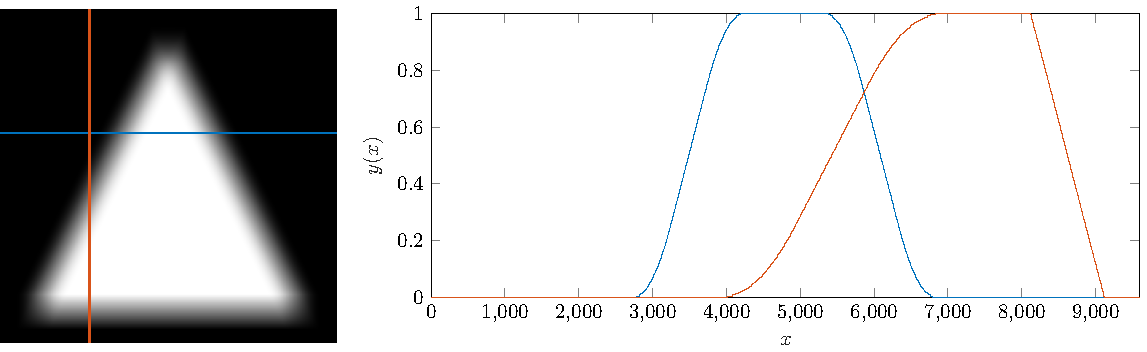
\includegraphics[width=0.9\textwidth]{./papers/deconvolve/pictures/dreieck.pdf}
\caption{Beispielbild und eindimensionale Interpretation\label{deconvolve:example}}
\end{figure}

Man folge in Abbildung \ref{deconvolve:example} beim Dreieck der blau markierten \glqq Zeile\grqq{}.
Reiht man diese Werte von links nach rechts auf, kommt man auf die blaue Kurve rechts in der Abbildung.
Analog kommt man auf die orange Kurve, wenn man der orangen \glqq Spalte\grqq{} folgt.
Vorteil diese Bildes ist also offensichtlich, dass man dessen zugehörige Matrix Zeilen- und Spaltenweise gleich wie das eindimensionale Signal betrachten kann.

Die Parameter $m$ und $\alpha$, die vorher für jedes Level einzeln bestimmt wurden, bleiben erhalten.
Die Funktion $s(cf_{k,n})$ aus \eqref{deconvolve:funktion} wird also auf alle Level gleich wie beim eindimensionalen Signal angewendet.
Dies geschieht einmal Zeilen- und Spaltenweise, es wird also insgesamt 19200 mal eine Analyse mit der diskreten Wavelet-Transformation durchgeführt.
Sind $f_\text{rows}(x,y)$ und $f_\text{cols}(x,y)$ die Zeilen-, bzw. Spaltenweise \glqq geschärften\grqq{} Varianten des ursprünglichen Bildes, kann davon das arithmetische Mittel genommen werden
$$f_\text{sharp}(x,y)=\frac{f_\text{rows}(x,y)+f_\text{cols}(x,y)}{2},$$
wobei $f_\text{sharp}(x,y)$ das so erhaltene Endresultat bezeichnet.

Nun ist zu erwarten dass die im vorherigen Abschnitt aufgetretenen Artefakte auch hier wieder in Erscheinung treten.
Abbildung \ref{deconvolve:ergebnis} zeigt das Ergebnis.
\begin{figure}[h]
\centering
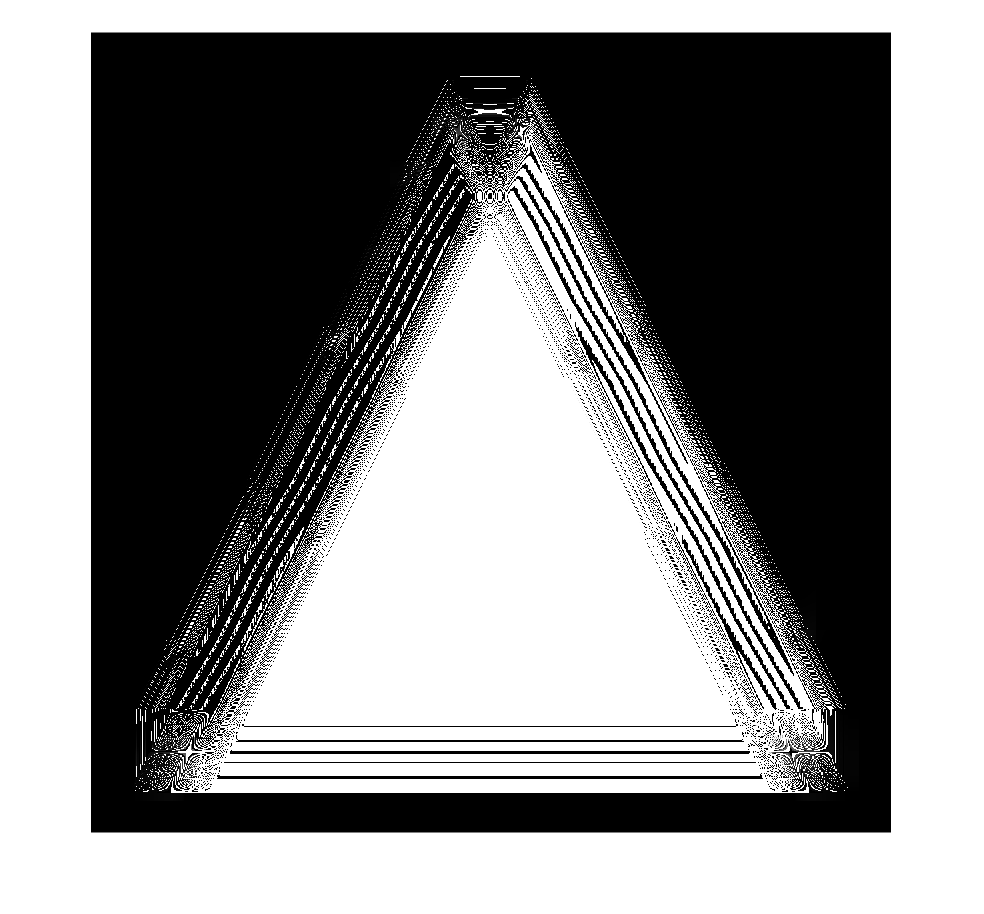
\includegraphics[width=0.7\textwidth]{./papers/deconvolve/pictures/dreieck_sharp.png}
\caption{Mit $s(cf_{k,n})$ \glqq geschärftes\grqq{} Bild\label{deconvolve:ergebnis}}
\end{figure}
 
Eine Verbesserung ist wie vorherzusehen nicht zu erkennen. Wo vorher der Rand verschwommen war, sind jetzt einfach starke Schwingungen aufgetaucht.